
\chapter{Simulation and Analysis tools}\label{mu2eana}

The Mu2e software framework is designed to study the expected performance of the Mu2e detectors, the signal 
reconstruction efficiency, and the characteristics of the backgrounds. The simulation framework is based on 
GEANT4, a widely used simulation toolkit. The simulation relies on Monte Carlo methods.

It is implemented in the C++ programming language and includes a comprehensive set of tools, such as 
tracking, geometry, and physics models. The library provides models of physical processes like particle 
scattering, energy loss, and decay of long-lived particles over a wide energy range. The simulation 
environment implements the Mu2e geometry. Pattern recognition and track reconstruction algorithms are 
incorporated into the software framework.

\section{art and FHiCL}

The Mu2e Offline software is based on the \textit{art} framework (Figure \ref{fig:multistage}). 
This framework is developed and maintained by the Fermilab Scientific 
Computing Division (SCD) and is used by multiple Intensity Frontier experiments at Fermilab.


\textit{art} is a command-line-driven event-processing framework written in 
C++. It operates in a non-interactive mode where it sequences events as directed 
by the user. It has been designed to fulfill a wide range of requirements in 
high-energy physics experiments, including high-level software triggers, online data 
monitoring, calibration, reconstruction, simulation, and analysis.


\textit{art} runtime configuration is written in the Fermilab Hierarchical 
Configuration Language (FHiCL), a data definition language developed at Fermilab. 
A FHiCL file contains definitions of C++ classes that implement the \textit{art} 
services. Within these classes, algorithms ranging from simulation and 
reconstruction to analysis codes are built and integrated into dynamic 
libraries called modules. The FHiCL files declare which modules will be loaded, 
in what order they will run, and which files will be read in input and written in output.


The simulation begins by using a FHiCL file to configure the process, specifying 
the necessary modules and call files containing essential geometry and physics data.

\section{STNTUPLE and ROOT}
STNTUPLE is an n-tuple data format and a lightweight n-tuple analysis framework, 
written (almost) exclusively in C++. It has been used for many years by the CDF experiment at Fermilab 
and ported to Mu2e. One of the plug-in modules for \textit{art} is specific to the 
usage of the STNTUPLE \cite{stntuple}. Every STNTUPLE file is a ROOT file containing multiple branches, 
each corresponding to a data block. A block is a data container optimized for I/O and 
analysis purposes, storing the Mu2e raw and/or reconstructed data. A STNTUPLE of the 
data saved in an \textit{art} file can be created and stored by using the appropriate 
module in the .fcl \textit{art}-job configuration file. The type of data saved in this 
format is customizable. Once the .stn file is generated, the analysis can be conducted 
using this data format, avoiding the re-running of the reconstruction. STNTUPLE is built 
on top of a data analysis and graphics package ROOT developed at CERN and allows the use 
of all interactive features of ROOT in the analysis.


\begin{figure}[!h]
    \centering
    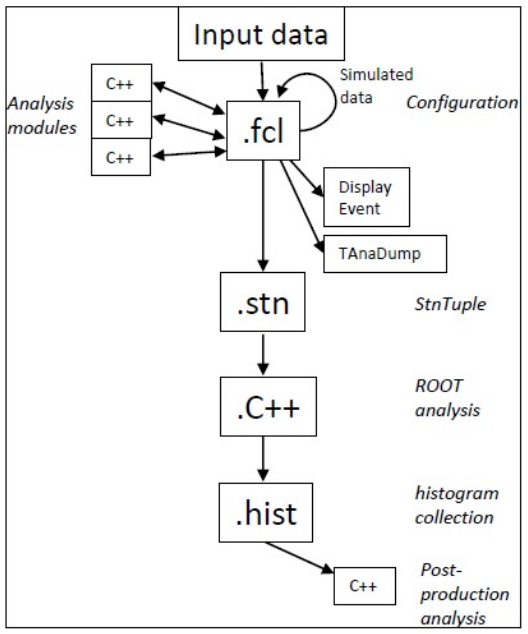
\includegraphics[width =0.4\textwidth]{figures/png/Screenshot_20240809_174458.png}
    \caption[Mu2e simulation and data handling.]{Both generation and reconstruction of events are done through art-jobs
    configured using FHiCLs and importing the necessary C++ modules. Other modules,
    like the Event Display and TAnaDump, are used for debugging purpose. The analysis
    workflow followed relies on the usage of STNTUPLE.}
    \label{fig:multistage}
\end{figure}

\section{Multi-stage Simulation}

Mu2e simulation employs a technique known as multi-stage simulation for efficient event 
generation and simulation. This approach involves 
generating and partially simulating events, 
pausing the simulation, and saving the generated data. Subsequent stages build upon this saved 
data, extending the simulation before saving again. Multiple stages may be utilized to complete 
a simulation. Stages can end when particles reach specific planes or volumes, such as the DS 
region containing the target and detector or the tracker volume. This method is particularly 
useful when early stages consume most of the CPU time in Mu2e simulations.

The motivations for using multi-stage simulation include:

\begin{itemize}
    \item \textbf{Progressive detector definition:} The simulation can define a portion of the 
    detector in later stages. For instance, computationally-intensive tasks like simulating 
    protons on target can be completed in an initial stage, allowing the tracker geometry and 
    algorithms to be inserted later. Once the tracker is ready, simulation can proceed into 
    its volume;
    \item \textbf{Efficient design variation studies:} It facilitates the study of different 
    experimental designs. Simulation stages can end outside a detector, enabling quick testing 
    of various detector designs with no need to repeat the entire prior simulation;
    \item \textbf{Effective error recovery:} It acts like a check-pointing mechanism, enhancing 
    error recovery efficiency. If an error occurs in a later stage, only that stage needs to be 
    redone using the output from the preceding stage. When early stages dominate CPU time, this 
    approach can lead to significant time savings;
    \item \textbf{Resource and limitation handling:} It can handle constraints like job duration 
    and output file size. Techniques like compression, event filtering, and concatenation can be 
    employed to manage resources effectively.
\end{itemize}

Multi-stage simulation also supports two other critical simulation techniques: mixing and resampling. 
These two techniques are necessary to study backgrounds and low statistics processes.

For the study of muon beamline vertical misalignments developed in this Thesis, the simulation 
framework consists of six stages:

\begin{itemize}
    \item \textbf{First stage (s1):} The interactions of 8 GeV protons in the Production Target (PT) 
    are simulated. All produced particles form the beam, which is traced up to the midpoint of the TS, 
    storing information about any particle that makes it that far;
    \item \textbf{Second stage (s2):} It uses the output of $s1$ and traces the beam up to the entrance 
    of the Detector Solenoid;
    \item \textbf{Third stage (s3):} It propagates the surviving particles from $s2$ through the 
    upstream portion of the DS vacuum and records muons stopped in the aluminum 
    Stopping Target (ST);
    \item \textbf{Fourth stage (s4):} $\mu^+$ and $\mu^-$ stopped in the ST are separated into two 
    different outputs for separate analysis;
    \item \textbf{Fifth stage (s5):} The detector is finally simulated. Target-stopped muons are 
    forced to undergo Michel decays. The resampling technique is employed to increase the available 
    statistics; each stopped muon is used several times as a starting point to generate different 
    decays. Particles that intersect the tracker or calorimeter are recorded;
    \item \textbf{Sixth stage (s6):} The simulated raw data are converted into simple C++ classes 
    or structs, simulating the digitization of detector raw data;
    \item \textbf{Seventh stage (s7):} The final stage reconstructs the particle tracks and 
    generates the n-tuples.
\end{itemize}

Multi-stage simulation saves computation resources in the study of vertical misalignment 
effects. The production of datasets with displaced COL3 requires only re-running from stage 
2 onwards. This is very convenient as $s1$ is the most resource-consuming one.
